\documentclass{article}
\usepackage[utf8]{inputenc}
\usepackage{amsmath}
\usepackage{graphicx}
\usepackage{enumerate}
\usepackage{pgfplots}
\usepackage{filecontents}
\usepackage{multirow}
\usepackage{booktabs}
\usepackage{subcaption}
\usepackage[margin=1in]{geometry}
\graphicspath{ {./} }

\title{CS6375 Final Project: Classifying Disaster Response Messages}
\author{Siddhant Sahu, Geetika Jain}

\setlength{\parindent}{0em}

\begin{document}
\maketitle

\begin{abstract}
We aim to tackle the problem of disaster management by building a text classifier to interpret and classify messages received during a disaster. We start by exploring the characteristics of the data, such as class imbalance, mean and median of message length, message length distribution, vocabulary etc. Our modeling approach involves exploring n-gram features and sequence based features to test the efficacy of machine learning algorithms. We also train a convolutional neural network and compare it with other machine learning models.
\end{abstract}

\section{Introduction}
The goal of disaster management is to protect or preserve the maximum number of lives and property during a natural disaster such as floods, cyclones, hurricanes or earthquakes. It can be defined as the organization and management of resources and responsibilities for dealing with all sorts of emergencies - preparedness, response and recovery in order to lessen the impact of disasters.
\\

With the increasing use of smartphones and networks, it has become possible for people affected by disasters to ask for help during a disaster, via communication channels such as national helplines, social media, etc. This also allows the authorities to make the most effective use of the resources in order to tend to the affected as soon as possible.
\\

Recent advances in machine learning and natural language processing have made it possible to classify the responses received into certain categories that aid the disaster management teams in allocating resources and teams.
\\

In this, we aim to build classifiers to classify messages into one or more categories. Examples include:

\begin{itemize}
	\item Call for aid
	\item Missing persons
	\item Medical help
	\item Need for clothing, water and food
	\item Reports of deaths
	\item Search and rescue operations
\end{itemize}

\section{Data}
The dataset\cite{dataset} contains 30,000 messages (covering multiple languages) drawn from events including an earthquake in Haiti in 2010, an earthquake in Chile in 2010, floods in Pakistan in 2010, super-storm Sandy in the U.S.A. in 2012, and news articles spanning a large number of years and 100s of different disasters.
\\

The data has been encoded with 36 different categories related to disaster response and has been stripped of messages with sensitive information in their entirety. We will work with the English translated version of the messages, for simplicity. For our experiments, we merge \texttt{disaster\_response\_messages\_training.csv} and \texttt{disaster\_response\_messages\_validation.csv} to create our training set. In the table given below are some of the summary statistics of the merge training set.
\\

\begin{table}[h]
	\centering
	\begin{tabular}{cc}
		\toprule
		\textbf{Description} & \textbf{Statistic} \\ 
		\midrule
		Number of relevant messages & 17720 \\ 
		Vocabulary & 13064 \\
		Average length of message (in words) & 13.5 \\
		Median length of message (in words) & 11 \\
		\bottomrule
	\end{tabular}
\caption{Summary statistics of merged training set}
\label{training-summary}
\end{table}

Note that stopwords and words occurring only once in the collection weren't considered towards calculating the above statistics.
\\

We next consider the distribution of \textit{class ratio} for the 36 categories present in the data. Higher the class ratio, more is the imbalance for the output column. Class ratio is computed as the number of samples of the majority class to the number of samples of the minority class. Thus, a class ratio of, say 150, could mean that there is only 1 negative example for 150 positive examples.

\begin{center}
	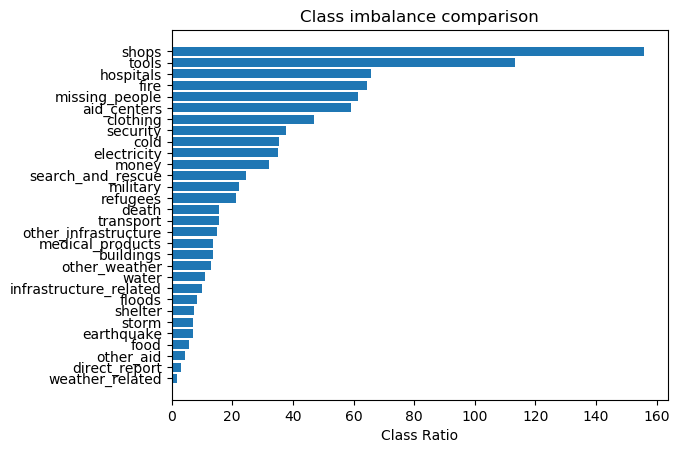
\includegraphics[scale=0.8]{class_ratio}
\end{center}

We will deal with classes with smaller class ratio to avoid the imbalanced classification problem. Working with imbalanced datasets is another problem in itself that calls for different approaches to modelling, e.g. undersampling, oversampling or framing it as an anomaly detection problem. Therefore, we avoid dealing with imbalanced classes.
\\

We next analyze the distribution of length of messages in the training data. For calculating the length of messages, we discount the stopwords and all other words that occur only once in the corpus. Moreover, we define length of a message as the number of tokens in the message. We tokenize the text using the \texttt{CountVectorizer} function in scikit-learn, which uses white-space tokenizer by default.

\begin{center}
	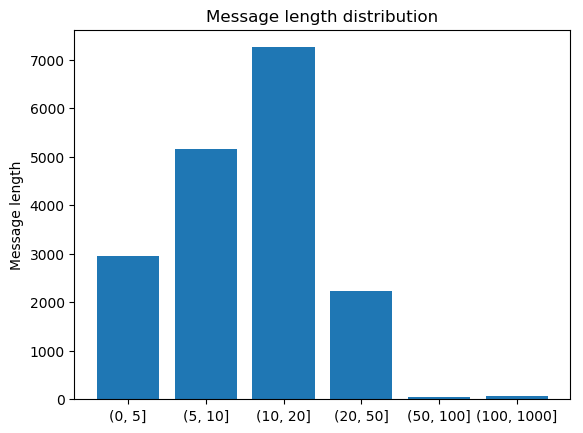
\includegraphics[scale=0.7]{sen_len_dist}
\end{center}

\section{Pre-processing}

\subsection{N-Gram Features}
For text data, the common practice is to first \textit{tokenize} the text and then convert the word tokens into vectors that machine learning algorithms can understand, also known as \textit{vectorizing} the text. The simplest method is to generate n-gram features and use one-hot encoding to build a count vector for each sentence. This is known as the \textit{bag of words} model where the sentence is considered a bag of words. For example, consider the sentence \texttt{Microsoft is the most valuable company}. Using unigrams ($n = 1$), the representation is \texttt{[`Microsoft', `is', `the', `most', `valuable', `company']}, using bigrams ($n = 2$), \texttt{[`Microsoft is', `is the', `the most', `most valuable', `valuable company']} and so on.
\\

Note that the actual vector can also be weighted using the TF-IDF weighting scheme which considers rare words as being more informative and commonly occurring words as being less informative. TF-IDF still doesn't consider sequence into account but generally performs much better than simply taking counts. 
\\

\textbf{Feature selection} The above method of vectorizing the text generates a lot of sparsity and the vector size grows with the vocabulary of the corpus. Not all the features in the vectors are important and don't contribute to the actual performance of the model. We select the top $K$ features using feature selection algorithms available in scikit-learn, such as \texttt{SelectKBest}. Feature selection serves two purposes -- it reduces the model complexity, hence bringing down the training time without sacrificing performance.

\subsection{Word Embeddings}
The bag-of-words model is an extremely simple representation of the text that doesn't usually carry more information. Words have meaning associated with them which again depends on the \textit{context} in which the word occurs. Context refers to a fixed window of surrounding words around the word in consideration. \texttt{word2vec} learns a dense representation of words in vector space by taking into consideration the context of the word.
\\

Previous research has suggested that this is able to learn semantic representations of words in vector space. \texttt{word2vec} also learns the most efficient representations of words. So, we can think of it as an automatic feature selection and dimensionality reduction algorithm where it learns a compact representation of the most useful features, like PCA.

\section{Approach}

\subsection{Evaluation}
For our experiments, we choose the \texttt{weather\_related} category with a class ratio of 1.69. We use \textit{f-score} to evaluate how well our classifier performs because accuracy fails when the classes are not balanced. This means we also tune our hyper-parameters based on f-scores. We also report the precision and recall scores for completeness. Note that in cases like search and rescue teams, precision might be more slightly important than recall. In such a case, a weighted version of the f-score would me more appropriate to evaluate the classifier. In general, choosing the right metric depends on the task at hand. However, for simplicity, we just use the default f-score that considers precision and recall equally important.

\subsection{Bag-of-Words Models}
First, we train models that do not consider the natural ordering of words. We generate n-gram features, as mentioned above, and train multi-layer perceptrons, support vector machines and gradient boosted trees on the feature vectors generated using TF-IDF weighting.

\subsection{Sequence Based Models}
We also train models which take sequence of the words into account. Generally, sequence based models have an additional embedding layer where we can pass our word vectors, such as those generated from \texttt{word2vec} algorithm or pre-trained word vectors. We limit this section to convolutional neural networks (CNNs). We train CNNs using \texttt{spaCy}, a natural language processing library, primarily because it provides convenient pipelines meant specifically for several NLP and text classification tasks.

\subsection{Hyperparameter optimization} We tune these models using several parameters using 5-fold cross-validation to test our performance. We then output the score the best estimator achieves on the test set.

\section{Experiment Results}

In Table \ref{ngram}, we show the results obtained in our training experiments on test data. We consider 5 different types of classifiers that are fundamentally different from one another to see how a family of classifiers would perform on the task. We use (i) Naive Bayes, a probabilistic classifier, (ii) SVM with linear kernel, a linear classifier, (iii) multi-layer perceptrons, i.e. neural networks, (iv) XGBoost, tree based ensemble model and (v) CNN, deep learning model.

%TODO: feature selection hurts performance of naive bayes
%TODO: experiment with PCA for feature selection

\begin{table}[h]
	\centering
	\begin{tabular}{cccc}
		\toprule
		\textbf{Model} & \textbf{Precision} & \textbf{Recall} & \textbf{F-score} \\ 
		\midrule 
		Naive Bayes & 0.56 & 0.66 & 0.61 \\ 
		SVM & 0.78 & 0.88 & 0.82 \\ 
		Multi-layer Perceptrons & 0.75 & 0.81 & 0.78 \\
		XGBoost & 0.76 & 0.92 & 0.83 \\ 
		CNN & 0.84 & 0.78 & 0.81 \\
		\bottomrule 
	\end{tabular} 
	\caption{Best results of classifiers}
	\label{ngram}
\end{table}

SVM achieves the best parameters using a linear kernel and a $C$ value of 1.0. It also proved to be the fastest among all the classifiers.
\\

Multi-layered perceptrons achieve the best score using 2 hidden layers with 50 neurons each, the \textit{relu} activation function with an \textit{adaptive} learning rate. One reason for the relatively poor performance of this could be the use of scikit-learn implementation\cite{sklearn}.
\\

XGBoost\cite{xgboost} turns out to be the best performing models that we tuned using a randomized search over a distribution of parameters. The best XGBoost model uses a learning rate of 0.37 and maximum depth of 6.
\\

\textbf{Using spaCy to train a CNN model} We use spaCy's recipe to put together a CNN text classifier\cite{spacy}. After training for 10 epochs, it is able to achieve a f-score of 0.81, but a precision of 0.84. The CNN model compresses the text vector by concatenating max and mean pooling, and uses the Adam solver with a learning rate of 0.001. It also uses a batch increasing technique, wherein it starts training with batch size of 1 and increases batch size to a specified maximum in a compounded fashion. The dropout rate is set to 0.2 to prevent overfitting.

\section{Conclusion}
In this project, we explored several machine learning models including deep learning approaches like CNNs. We saw that bag-of-words models achieve decent scores on this dataset and are faster to train than CNN (at least on CPUs). However, we hypothesize that CNNs would be able to outperform the bag-of-words model given more data and compute power.
\\

Nevertheless, this is an indication that building and deploying such a text classification system can still be effective in managing the situation during a natural disaster.

\begin{thebibliography}{1}
	
	\bibitem{sklearn} Scikit-Learn \texttt{https://scikit-learn.org/stable/user\_guide.html}
	
	\bibitem{dataset} Multilingual disaster response messages \texttt{https://www.figure-eight.com/dataset/combined-disaster-response-data/}
	
	\bibitem{xgboost} XGBoost \texttt{https://xgboost.readthedocs.io/en/latest/index.html}
	
	\bibitem{spacy} Spacy text classification using CNN \texttt{https://spacy.io/usage/}
	
\end{thebibliography}

\end{document}